\documentclass[11pt, a4paper, fleqn]{article}

\usepackage[portuguese]{babel}
\usepackage{graphicx}
\usepackage{leading}
\usepackage{tabularx}
\usepackage{geometry}
\usepackage[utf8]{inputenc}
\usepackage{booktabs}
\usepackage{array}
\usepackage{xcolor}
\usepackage{tikz}
\usetikzlibrary{calc}
\usepackage{eso-pic}
\usepackage{listings}
\usepackage{listingsutf8}


%----------------- font -------------------------------------------------------%
\usepackage[T1]{fontenc}
\usepackage{paratype}
\usepackage[basic, italic]{mathastext}

%----------------- titles formats ---------------------------------------------%
\usepackage{titlesec}
\titleformat{\part}
{\LARGE\bfseries}{\thepart}{1em}{}
\titleformat{\section}
{\LARGE\bfseries}{\thesection}{1em}{}
\titleformat{\subsection}
{\Large\bfseries}{\thesubsection}{1em}{}
\titleformat{\paragraph}[runin]
{\sffamily\bfseries}
{}
{0pt}
{}

%----------------- footnote format --------------------------------------------%
\usepackage[perpage, bottom, marginal]{footmisc}
\makeatletter
\renewcommand{\@makefnmark}{\hbox{\textsuperscript{\sffamily\@thefnmark}}}
\makeatother
\renewcommand*{\footnotelayout}{\footnotesize\sffamily}

%----------------- page number format -----------------------------------------%
\usepackage{fancyhdr}
\fancypagestyle{pagestyle}{%
	\fancyhf{}
	\fancyfoot[C]{\makebox[\textwidth]{\sffamily\normalsize\thepage}}
	\renewcommand{\headrulewidth}{0pt}
	\renewcommand{\footrulewidth}{0pt}
}

%----------------- verbatim ---------------------------------------------------%
\usepackage{fancyvrb}


\definecolor{coverbar}{HTML}{263238}

\newcommand{\Titulo}{Punch Card}
\newcommand{\UC}{Processamento de Linguagens}
\newcommand{\Sigla}{PL}
\newcommand{\Grupo}{09}
\newcommand{\AnoLetivo}{2025/2026}

\newcommand{\listaAlunos}{%
	\aluno{A106919}{Eduardo Freitas Fernandes}\\[6pt]%
	\aluno{A106842}{Gonçalo Rodrigues Ribeiro}\\[6pt]%
	\aluno{A106888}{José Mário Raimundo Lima}%
}


\newcommand{\aluno}[2]{%
	\makebox[2.5cm][l]{\textbf{#1}}#2%
}

\newcommand{\logobox}[1]{%
	\IfFileExists{#1}{%
		\includegraphics[width=26mm,keepaspectratio]{#1}%
	}{%
		\setlength{\fboxsep}{0pt}%
		\colorbox{gray!25}{\makebox[26mm][c]{\rule{0pt}{18mm}\small\textsf{#1}}}%
	}%
}

\newcommand{\makecover}{
	\newgeometry{left=4.5cm, right=3cm, top=4cm, bottom=3cm}
	\thispagestyle{empty}
	
	\AddToShipoutPictureBG*{
		\begin{tikzpicture}[remember picture, overlay]
			\fill[coverbar]
			(current page.north west)
			rectangle
			($(current page.south west) + (2.5cm, 0)$);
			\node[
			anchor    = south east,
			inner sep = 0pt,
			xshift    = -3cm,
			yshift    =  3cm,
			font      = \fontsize{70}{70}\selectfont\bfseries\sffamily,
			text      = coverbar,
			] at (current page.south east) {\Sigla};
		\end{tikzpicture}
	}
	
	\begingroup
	\raggedright
	\setlength{\parindent}{0pt}
	
	\logobox{imgs/UM.jpg}\logobox{imgs/EE.jpg}
	\par\vspace{7mm}
	
	{\fontsize{14.4pt}{17pt}\selectfont\textbf{Universidade do Minho}\par}
	{\fontsize{14.4pt}{17pt}\selectfont Escola de Engenharia\par}
	{\fontsize{14.4pt}{17pt}\selectfont Licenciatura em Engenharia Informática\par}
	
	\vspace{50mm}
	
	{\fontsize{30pt}{24pt}\selectfont\textbf{\Titulo}\par}
	\vspace{1.5em}
	{\fontsize{20pt}{24pt}\selectfont\UC\par}
	{\fontsize{17pt}{21pt}\selectfont Ano Letivo \AnoLetivo\par}
	
	\vspace{45mm}
	
	{\fontsize{14.4pt}{18pt}\selectfont\textbf{Grupo \Grupo}\par}
	\vspace{10pt}
	{\fontsize{14.4pt}{18pt}\selectfont\listaAlunos\par}
	
	\endgroup
	\restoregeometry
	\clearpage
}

\lstset{
  basicstyle=\ttfamily\small,
  breaklines=true,
  frame=single,
  captionpos=b,
}

\begin{document}
\sffamily
\setlength{\parindent}{0em}
\emergencystretch 3em
\renewcommand{\baselinestretch}{1.25}

\makecover

\newgeometry{left=25mm,right=20mm,top=25mm,bottom=25mm}
\setlength{\parindent}{1em}

\tableofcontents

\newpage

% ─────────────────────────────────────────────────────────────────────────────
\section{Introdução}

\noindent Este relatório descreve o desenvolvimento do compilador PunchCard, realizado no âmbito da unidade curricular de Processamento de Linguagens do ano letivo 2025/2026. O objetivo do projeto foi implementar um compilador completo para a linguagem Fortran 77 (standard ANSI X3.9-1978), capaz de traduzir código Fortran para instruções da máquina virtual EWVM disponibilizada. O compilador foi desenvolvido em Python, utilizando a biblioteca \texttt{ply} para a construção do analisador léxico e sintático. A implementação cobre todas as etapas obrigatórias, análise léxica, sintática, semântica e geração de código, bem como a implementação de funções e subrotinas.

\section{Arquitetura do Sistema}

O compilador está organizado em quatro módulos principais, cada um responsável por uma fase distinta da compilação. O fluxo de execução é sequencial: a saída de cada fase é a entrada da seguinte.

\begin{figure}[h]
    \centering
    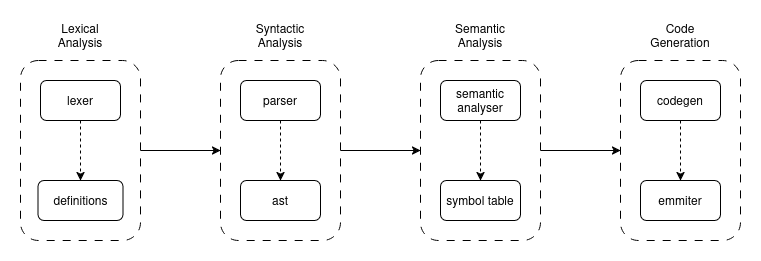
\includegraphics[width=0.7\linewidth]{imgs/arquitetura.png}
    \caption{Arquitetura do compilador PunchCard.}
    \label{fig:arquitetura}
\end{figure}

\subsection{Análise Léxica (\texttt{lexer/})}

O analisador léxico converte o código-fonte Fortran numa sequência de \textit{tokens}. Foi implementado com \texttt{ply.lex} no módulo \texttt{lexer/lexer.py}, com as definições de tokens em \texttt{lexer/definitions.py}. Os tokens reconhecidos incluem:

\begin{itemize}
    \item \textbf{\textit{Keywords}:} \texttt{PROGRAM}, \texttt{INTEGER}, \texttt{REAL}, \texttt{LOGICAL}, \texttt{CHARACTER}, \texttt{DOUBLE PRECISION}, \texttt{IF}, \texttt{THEN}, \texttt{ELSE}, \texttt{ENDIF}, \texttt{DO}, \texttt{CONTINUE}, \texttt{GOTO}, \texttt{PRINT}, \texttt{READ}, \texttt{FUNCTION}, \texttt{SUBROUTINE}, \texttt{RETURN}, \texttt{CALL}, \texttt{END}.
    \item \textbf{Valores Literais:} inteiros (\texttt{LIT\_INT}), reais (\texttt{LIT\_FLOAT}), dupla precisão (\texttt{LIT\_DOUBLE}), strings (\texttt{LIT\_STRING}) e booleanos (\texttt{LIT\_BOOLEAN}, i.e., \texttt{.TRUE.} e \texttt{.FALSE.}).
    \item \textbf{Operadores relacionais e lógicos:} \texttt{.EQ.}, \texttt{.NE.}, \texttt{.LT.}, \texttt{.LE.}, \texttt{.GT.}, \texttt{.GE.}, \texttt{.AND.}, \texttt{.OR.}, \texttt{.NOT.}.
    \item \textbf{Identificadores} e caracteres literais simples: \texttt{( ) , = + - * /}.
\end{itemize}

\noindent O lexer opera em formato livre (\textit{free-form}), ignorando espaços e tabulações. Os identificadores e palavras-chave são tratados de forma \textit{case-insensitive}, tudo é convertido para maiúsculas internamente.

\subsection{Análise Sintática (\texttt{parser/})}

O analisador sintático valida a estrutura gramatical do programa e constrói a Árvore Sintática Abstrata (AST). Foi implementado com \texttt{ply.yacc} no módulo \texttt{parser/parser.py}, com os nós da AST definidos em \texttt{parser/ast.py}. A gramática suporta:

\begin{itemize}
    \item Programas principais (\texttt{PROGRAM ... END}) e subprogramas (\texttt{FUNCTION}, \texttt{SUBROUTINE}).
    \item Declarações de variáveis escalares e arrays.
    \item Atribuições, expressões aritméticas, relacionais e lógicas.
    \item Estruturas de controlo: \texttt{IF-THEN-ELSE-ENDIF}, \texttt{IF} inline, ciclos \texttt{DO} com e sem passo, \texttt{GOTO}.
    \item Operações de I/O: \texttt{PRINT} e \texttt{READ}.
    \item Chamadas de subrotinas (\texttt{CALL}) e funções como expressão.
\end{itemize}

\noindent A precedência de operadores é declarada explicitamente no parser, seguindo a hierarquia do Fortran 77: potência tem maior precedência, seguida de multiplicação/divisão, adição/subtração, operadores relacionais e por fim lógicos.

\subsection{Análise Semântica (\texttt{semantic/})}

O analisador semântico percorre a AST e verifica a coerência do programa. É implementado com o padrão \textit{Visitor}, no módulo \texttt{semantic/semantic\_analyser.py}. A tabela de símbolos está em \texttt{semantic/symbol\_table.py}. As verificações realizadas incluem:

\begin{itemize}
    \item \textbf{Declaração de variáveis:} uso de variáveis não declaradas é reportado como erro.
    \item \textbf{Tipos:} verificação de compatibilidade de tipos em atribuições e operações. Coerções implícitas entre tipos numéricos (INTEGER, REAL, DOUBLE PRECISION) são permitidas, com aviso.
    \item \textbf{Arrays:} verificação do número de índices na declaração e no acesso.
    \item \textbf{Labels DO/CONTINUE:} o label do \texttt{DO} tem de coincidir com o do \texttt{CONTINUE} correspondente.
    \item \textbf{Subprogramas:} verificação do número de argumentos em chamadas de funções e subrotinas.
    \item \textbf{Resolução de ambiguidade:} a sintaxe \texttt{nome(args)} é ambígua entre acesso a array e as chamadas de funções. O analisador semântico resolve esta ambiguidade consultando a tabela de símbolos e reclassifica o nó da AST em conformidade.
\end{itemize}

\subsection{Geração de Código (\texttt{codegen/})}

O gerador de código percorre a AST e emite instruções EWVM. É também implementado com o padrão \textit{Visitor}, no módulo \texttt{codegen/codegen.py}. O módulo \texttt{codegen/emitter.py} acumula as instruções e produz o código final como texto. As principais decisões de geração de código são descritas na secção seguinte.

\section{\textit{Context Free Grammar}}

\subsection{Programa e Unidades de Programa}

\begin{lstlisting}
program : program_unit_list

program_unit_list : program_unit
                  | program_unit_list program_unit

program_unit : main_program
             | function_subprogram
             | subroutine_subprogram

main_program : PROGRAM IDENTIFIER body END

function_subprog : type_spec FUNCTION IDENTIFIER '(' param_list ')' body END

subroutine_subprog : SUBROUTINE IDENTIFIER '(' param_list ')' body END
\end{lstlisting}

\noindent A lista de unidades de programa usa recursividade à esquerda para otimizar o funcionamento do \textit{parser} LALR(1) do PLY, evitando crescimento desnecessário da pilha. O compilador interpreta um programa como um conjunto de unidades independentes, cada uma delimitada pelo seu cabeçalho e pelo \textit{token} de encerramento correspondente.

\subsection{Corpo do Programa e Declarações}

\begin{lstlisting}
body : declaration_section statement_section
declaration_section : declaration_section declaration
                    |

declaration : type_spec var_list
type_spec : DT_INTEGER
          | DT_REAL
          | DT_DOUBLE_PRECISION
          | DT_LOGICAL
          | DT_CHARACTER

var_list : var_decl
         | var_list ',' var_decl

var_decl : IDENTIFIER
         | IDENTIFIER '(' dim_list ')'

dim_list : expr
         | dim_list ',' expr
\end{lstlisting}

\noindent O corpo do programa impõe que todas as variáveis sejam declaradas antes das instruções. A produção vazia permite subprogramas sem declarações explícitas. A regra de declaração unifica variáveis escalares e \textit{arrays}, validando dimensões como expressões.

\subsection{Instruções e \textit{Labels}}

\begin{lstlisting}
statement_section : statement_section statement
                  |

statement : LIT_INT statement_body
          | statement_body

statement_body : assignment_stmt
               | goto_stmt
               | if_stmt
               | do_stmt
               | continue_stmt
               | print_stmt
               | read_stmt
               | stop_stmt
               | return_stmt
               | call_stmt

assignment_stmt : lvalue '=' expr

lvalue : IDENTIFIER
       | IDENTIFIER '(' arg_list ')'
\end{lstlisting}

\noindent Qualquer instrução pode ser precedida por um literal inteiro, representando \textit{labels} usadas em desvios e ciclos. A ambiguidade entre chamadas de função e acessos a arrays é mantida na gramática e resolvida apenas na análise semântica através da tabela de símbolos.

\subsection{Estruturas Condicionais}

\begin{lstlisting}
if_stmt : IF '(' expr ')' THEN statement_section ENDIF
        | IF '(' expr ')' THEN statement_section ELSE statement_section ENDIF
        | IF '(' expr ')' statement_body
\end{lstlisting}

\noindent A gramática inclui a ambiguidade clássica do \textit{dangling else}. O PLY resolve automaticamente o conflito através de shift, associando o \texttt{ELSE} ao \texttt{IF} mais interno, garantindo o comportamento esperado.

\newpage

\subsection{Ciclos DO}

\begin{lstlisting}
do_stmt : DO LIT_INT IDENTIFIER '=' expr ',' expr do_body
        | DO LIT_INT IDENTIFIER '=' expr ',' expr ',' expr do_body

do_body : do_inner_stmts LIT_INT CONTINUE

do_inner_stmts : do_inner_stmts do_inner_statement
               |

do_inner_statement : assignment_stmt | goto_stmt | if_stmt | do_stmt 
                   | print_stmt | read_stmt | stop_stmt | return_stmt | call_stmt
                   | LIT_INT assignment_stmt | LIT_INT goto_stmt | LIT_INT if_stmt 
                   | LIT_INT do_stmt | LIT_INT print_stmt | LIT_INT read_stmt 
                   | LIT_INT stop_stmt | LIT_INT return_stmt | LIT_INT call_stmt
\end{lstlisting}

\noindent O corpo do \texttt{DO} é isolado numa regra própria para garantir que o ciclo termina na \textit{label} indicada e que a instrução \texttt{CONTINUE} finaliza corretamente o bloco. Esta separação evita reduções prematuras e mantém o \textit{parser} estável.

\subsection{Entrada, Saída e Listas de Argumentos}

\begin{lstlisting}
continue_stmt : CONTINUE
print_stmt : PRINT '*' ',' output_list
           | PRINT LIT_STRING ',' output_list
           | PRINT '*'

read_stmt : READ '*' ',' input_list
          | READ '*'

stop_stmt : STOP
return_stmt : RETURN
call_stmt : CALL IDENTIFIER '(' arg_list ')'

param_list : param_list_mult |
param_list_mult : IDENTIFIER | param_list_mult ',' IDENTIFIER

arg_list : arg_list_mult |
arg_list_mult : expr | arg_list_mult ',' expr

output_list : expr | output_list ',' expr
input_list : lvalue | input_list ',' lvalue
\end{lstlisting}

\noindent A gramática distingue listas de parâmetros formais das listas de argumentos reais, ambas permitindo ausência de elementos. As instruções de leitura e escrita suportam o formato simples (\texttt{*}).

\subsection{Expressões}

\begin{lstlisting}
expr : logical_expr

logical_expr : logical_expr LOP_OR logical_and
             | logical_and

logical_and : logical_and LOP_AND logical_not
            | logical_not

logical_not : LOP_NOT logical_not
            | comparison

comparison : comparison rel_op arith_expr
           | arith_expr

rel_op : LOP_EQ | LOP_NE | LOP_LE | LOP_LT | LOP_GE | LOP_GT

arith_expr : arith_expr arith_op term
           | term

arith_op : '+' | '-'

term : term term_op factor
     | factor

term_op : '*' | '/'

factor : unary OP_POWER factor
       | unary

unary : '-' unary
      | '+' unary
      | primary

primary : '(' expr ')'
        | LIT_INT | LIT_FLOAT | LIT_DOUBLE
        | LIT_STRING | LIT_BOOLEAN
        | IDENTIFIER
        | IDENTIFIER '(' arg_list ')'
\end{lstlisting}

\noindent A hierarquia das expressões segue a precedência natural dos operadores, da lógica até aos elementos primários. A recursividade à esquerda garante associatividade correta para operações aditivas e multiplicativas, enquanto a potenciação usa recursividade à direita para refletir a sua associatividade natural. Literais, variáveis e expressões entre parênteses formam a base da precedência.

\section{Decisões de Implementação}

\subsection{Uso de AST e padrão \textit{Visitor}}

Optámos por construir uma AST explícita em vez de gerar código diretamente durante o parsing. Isto permitiu separar claramente as fases de análise semântica e geração de código, tornando o compilador mais fácil de testar e estender. \\

\noindent Tanto o analisador semântico como o gerador de código implementam o padrão \textit{Visitor}: cada nó da AST tem um método \texttt{accept(visitor)} que invoca o método correspondente no visitante (e.g., \texttt{visit\_IfStmt}, \texttt{visit\_DoStmt}). Isto evita misturar lógica de múltiplas fases no mesmo código.

\subsection{Estruturas de controlo}

\paragraph{Ciclo DO.}
O ciclo \texttt{DO} em Fortran 77 tem a forma \texttt{DO label var = start, stop [, step]}, terminando num \texttt{label CONTINUE}. Na geração de código, o ciclo é traduzido para:

\begin{enumerate}
    \item Inicialização da variável de controlo.
    \item Label de início do ciclo.
    \item Teste de condição (\texttt{var <= stop}).
    \item salto condicional para o fim se falso.
    \item Corpo do ciclo.
    \item Incremento da variável de controlo (passo 1 por omissão).
    \item Salto incondicional para o início.
    \item Label de fim do ciclo.
\end{enumerate}

\paragraph{IF.}
O \texttt{IF} bloco (\texttt{IF-THEN-ELSE-ENDIF}) e o \texttt{IF} inline são tratados de forma uniforme. Na geração de código, geram-se dois labels internos (\textit{ifelse} e \textit{ifend}) para controlar o fluxo com instruções \texttt{JZ} e \texttt{JUMP}.

\paragraph{GOTO.}
O \texttt{GOTO} é traduzido diretamente para \texttt{JUMP lN}, onde \texttt{N} é o label numérico do Fortran. Os statements com label emitem o label correspondente no início.

\subsection{Funções e Subrotinas}

O suporte a subprogramas foi implementado como valorização. Funções e subrotinas são emitidas após o programa principal, cada uma com o seu label.

\paragraph{Funções.}
Em Fortran 77, o valor de retorno de uma função é atribuído a uma variável com o mesmo nome da função (e.g., \texttt{CONVRT = VAL}). Essa variável é declarada implicitamente no início do frame da função. Na chamada, é reservado espaço no stack para o valor de retorno antes de adicionar os argumentos.

\paragraph{Subrotinas.}
As subrotinas não devolvem valor. São invocadas com \texttt{CALL}, e os argumentos são limpos do stack após o retorno.

\paragraph{Passagem de argumentos.}
Os argumentos são passados por valor, são colocados na \textit{stack} antes da chamada. Dentro do subprograma, são acedidos como locais negativos relativamente ao \textit{frame pointer} (\texttt{PUSHL} com índice negativo).

\subsection{Resolução da ambiguidade array/função}

A sintaxe \texttt{nome(args)} é sintacticamente idêntica para acessos a \textit{arrays} e para chamadas de funções. O \textit{parser} produz sempre um nó \texttt{ArrayAccess}. O analisador semântico, ao visitar esse nó, consulta a tabela de símbolos: se \texttt{nome} for uma função, reclassifica o nó para \texttt{FunctionCall} e ajusta os atributos. O gerador de código trata os dois casos de forma distinta.

\subsection{Funções built-in}

As funções intrínsecas \texttt{MOD}, \texttt{SIN} e \texttt{COS} são tratadas diretamente no gerador de código, mapeando para as instruções EWVM correspondentes (\texttt{MOD}, \texttt{FSIN}, \texttt{FCOS}), sem necessitar de declaração explícita.

\subsection{Tipos numéricos e coerção}

A hierarquia de tipos numéricos seguida é: \texttt{INTEGER} < \texttt{REAL} < \texttt{DOUBLE PRECISION}. Em operações mistas, o resultado é promovido para o tipo mais alto. Atribuições com coerção implícita são permitidas mas geram um aviso semântico.

\section{Manual de Utilização}

\subsection{Requisitos}

\begin{itemize}
    \item Python 3.10 ou superior.
    \item Dependências listadas em \texttt{requirements.txt} (instalar com \texttt{pip install -r requirements.txt}).
\end{itemize}

\subsection{Compilar um programa Fortran}

Para compilar um ficheiro \texttt{.f} e obter o código EWVM, deverá dirigir-se à pasta \texttt{src} e executar:

\begin{lstlisting}[language=bash]
python -m punchcard.main <ficheiro.f>
\end{lstlisting}

\noindent Exemplo:

\begin{lstlisting}[language=bash]
python -m punchcard.main ../test/basic/01_hello.f
\end{lstlisting}

\noindent O código EWVM é impresso para o \textit{stdout}. Em caso de erros léxicos, sintáticos ou semânticos, são impressas mensagens de erro com número de linha e coluna, e o compilador termina sem gerar código.

\noindent Também é possível passar código pelo \textit{stdin}:

\begin{lstlisting}[language=bash]
cat programa.f | python -m punchcard.main
\end{lstlisting}

\subsection{Executar os testes}

O script \texttt{run\_tests.sh} corre todos os testes e mostra o resultado:

\begin{lstlisting}[language=bash]
bash run_tests.sh all
\end{lstlisting}

\noindent Podem também ser executados grupos específicos:

\begin{lstlisting}[language=bash]
bash run_tests.sh basic   # exemplos do enunciado
bash run_tests.sh custom  # testes de funcionalidades individuais
\end{lstlisting}

\subsection{Estrutura do repositório}

\begin{itemize}
    \item \texttt{src/punchcard/} - código-fonte do compilador.
    \item \texttt{test/basic/} - os 5 exemplos do enunciado.
    \item \texttt{test/custom/} - testes de funcionalidades específicas.
    \item \texttt{docs/} - relatório técnico.
    \item \texttt{assets/} - enunciado do trabalho prático.
    \item \texttt{CFG.md} - \textit{Context Free Grammar}.
    \item \texttt{EWVM.md} - linguagem baseada em pilhas da máquina virtual.
    \item \texttt{run\_tests.sh} - \textit{script} para execução dos testes.
\end{itemize}

\section{Conclusão}

O compilador PunchCard implementa com sucesso todas as etapas obrigatórias do enunciado, bem como a valorização de subprogramas. Todos os exemplos do enunciado são compilados e produzem o resultado correto, e os 11 testes adicionais passam sem falhas. As principais dificuldades encontradas foram:

\begin{itemize}
    \item A \textbf{ambiguidade entre acesso a array e chamada de função}: resolvida na fase semântica com reclassificação dos nós da AST.
    \item O \textbf{mecanismo de retorno de funções} em Fortran 77, onde o valor de retorno é atribuído a uma variável com o mesmo nome da função, exigiu tratamento especial tanto na tabela de símbolos como na geração de código.
    \item A \textbf{passagem de argumentos} a subprogramas, incluindo a indexação correta relativa ao \textit{frame pointer}.
\end{itemize}

\noindent No geral, o projeto permitiu consolidar os conceitos de processamento de linguagens, desde a especificação léxica e gramatical até à geração de código para uma máquina virtual real.

\end{document}